\documentclass[12]{article}
\usepackage{graphicx} % this is for insert image
\usepackage{subcaption} %this is for multiple images
\usepackage[backend=bibtex, sorting=none]{biblatex} %this is needed for bibliograhy for rnw

\bibliography{ResearchProp} % name of my bibtex

% echo=F>>=
% opts_chunk$set(echo=F,message=F,warning=F)
% @

\title{Research proposal: Neighbordhood environment and obesity}
\date{2019-01-26}
\author{Kenta Okuyama}


\usepackage{Sweave}
\begin{document}
\Sconcordance{concordance:ne_cardio.tex:ne_cardio.Rnw:%
1 16 1 1 0 18 1 1 71 89 1}

\pagenumbering{gobble} %Gobble pagenumber in title page
\maketitle
\tableofcontents
\newpage
\pagenumbering{arabic}
  
\section{Introduction} %Biggest section
\paragraph{}
Obesity can lead to serious negative consequences, such as type 2 diabetes and cardiovascular disease, and its prevalnce has been increasing worldwide \cite{ng2014global,flegal2002prevalence}. Environmental and policy interventions are now recognized as an urgent approach to combat the global obesity epidemic \cite{gortmaker2011changing}. Although numerous research have been done on the influence of environmental features on obesity, there is no consistent evidence \cite{papas2007built,mackenbach2014obesogenic}. One of the major challenges is that majority of the studies were conducted cross-sectionally, thereby causal relationship has not been elucidated yet. A few recent studies found a significant association between neighborhood  physical environment features and obesity \cite{mason2018associations,barrientos2017neighborhood}. For example, Mason et al. found that both density of physical activity facilities and proximity to fastfood outlets were associated with adiposity in the expected direction among nation-wide adults cohort in UK. Barrientos et al. found that improvement of neighborhood enviroment in promoting both healthy eating and physical activity was related to BMI reduction among obese persons \cite{barrientos2017neighborhood}. This was the first preliminary finding for the association between longitudinal changes of physical environment and BMI. However, despite these recent findings, the association between neighborhood physical environment and obesity are still unclear \cite{nieuwenhuijsen2018influence}. This is mainly because complex mechanism for the incidence of obesity due to numerous factors that can affect energy inbalance for diet and physical activity, such as socio-economic status, neighborhood deprivation, and genetic risk factors (Figure 1). Lacking or inappropriate control for any of these factors would lead biased findings for the influence of neighborhood environment on obesity. Those recent studies were either lacking of control for any of the factors, such as neighborhood deprivation, or were conducted corss-sectionally. 
\paragraph{}
As another reason why the association between neighborhood envrionment and obesity is unclear, there are often umeasured factors that could infulence obesity within neighborhood studies. For example, there is a growing body of evidences that not only physical environment, but also social environments might affect on physical activity and obeisty through different pathways \cite{carrillo2019neighbourhood,suglia2016neighborhood}. Social environments are often measured by social capital which refers to mutual trust, supports, and participation of social activity among neighborhoods \cite{kawachi1997social}. Several studies have examined the association between social capital and obesity, yet envidence for this association has been inconsistent \cite{carrillo2019neighbourhood}. A few studies have investigated whether neighborhood social capital and physical environment was associated to each other, but these findings are also inconsistent \cite{leyden2003social,hanibuchi2012does}. Although both physical environment and social environment are factors in the upstream for the obesity related behaviors, few studies have examined which factor affect on obesity more than the other. From these background, this study consists of two aims.

\paragraph{Aim 1}
Examine the longitudinal association between changes in neighborhood physical environment (food and physical activity) and obesity.
\paragraph{Aim 2}
Examine the association between neighborhood physical environment and its interaction with social environment on obesity.


\begin{figure}[h!]
\centering
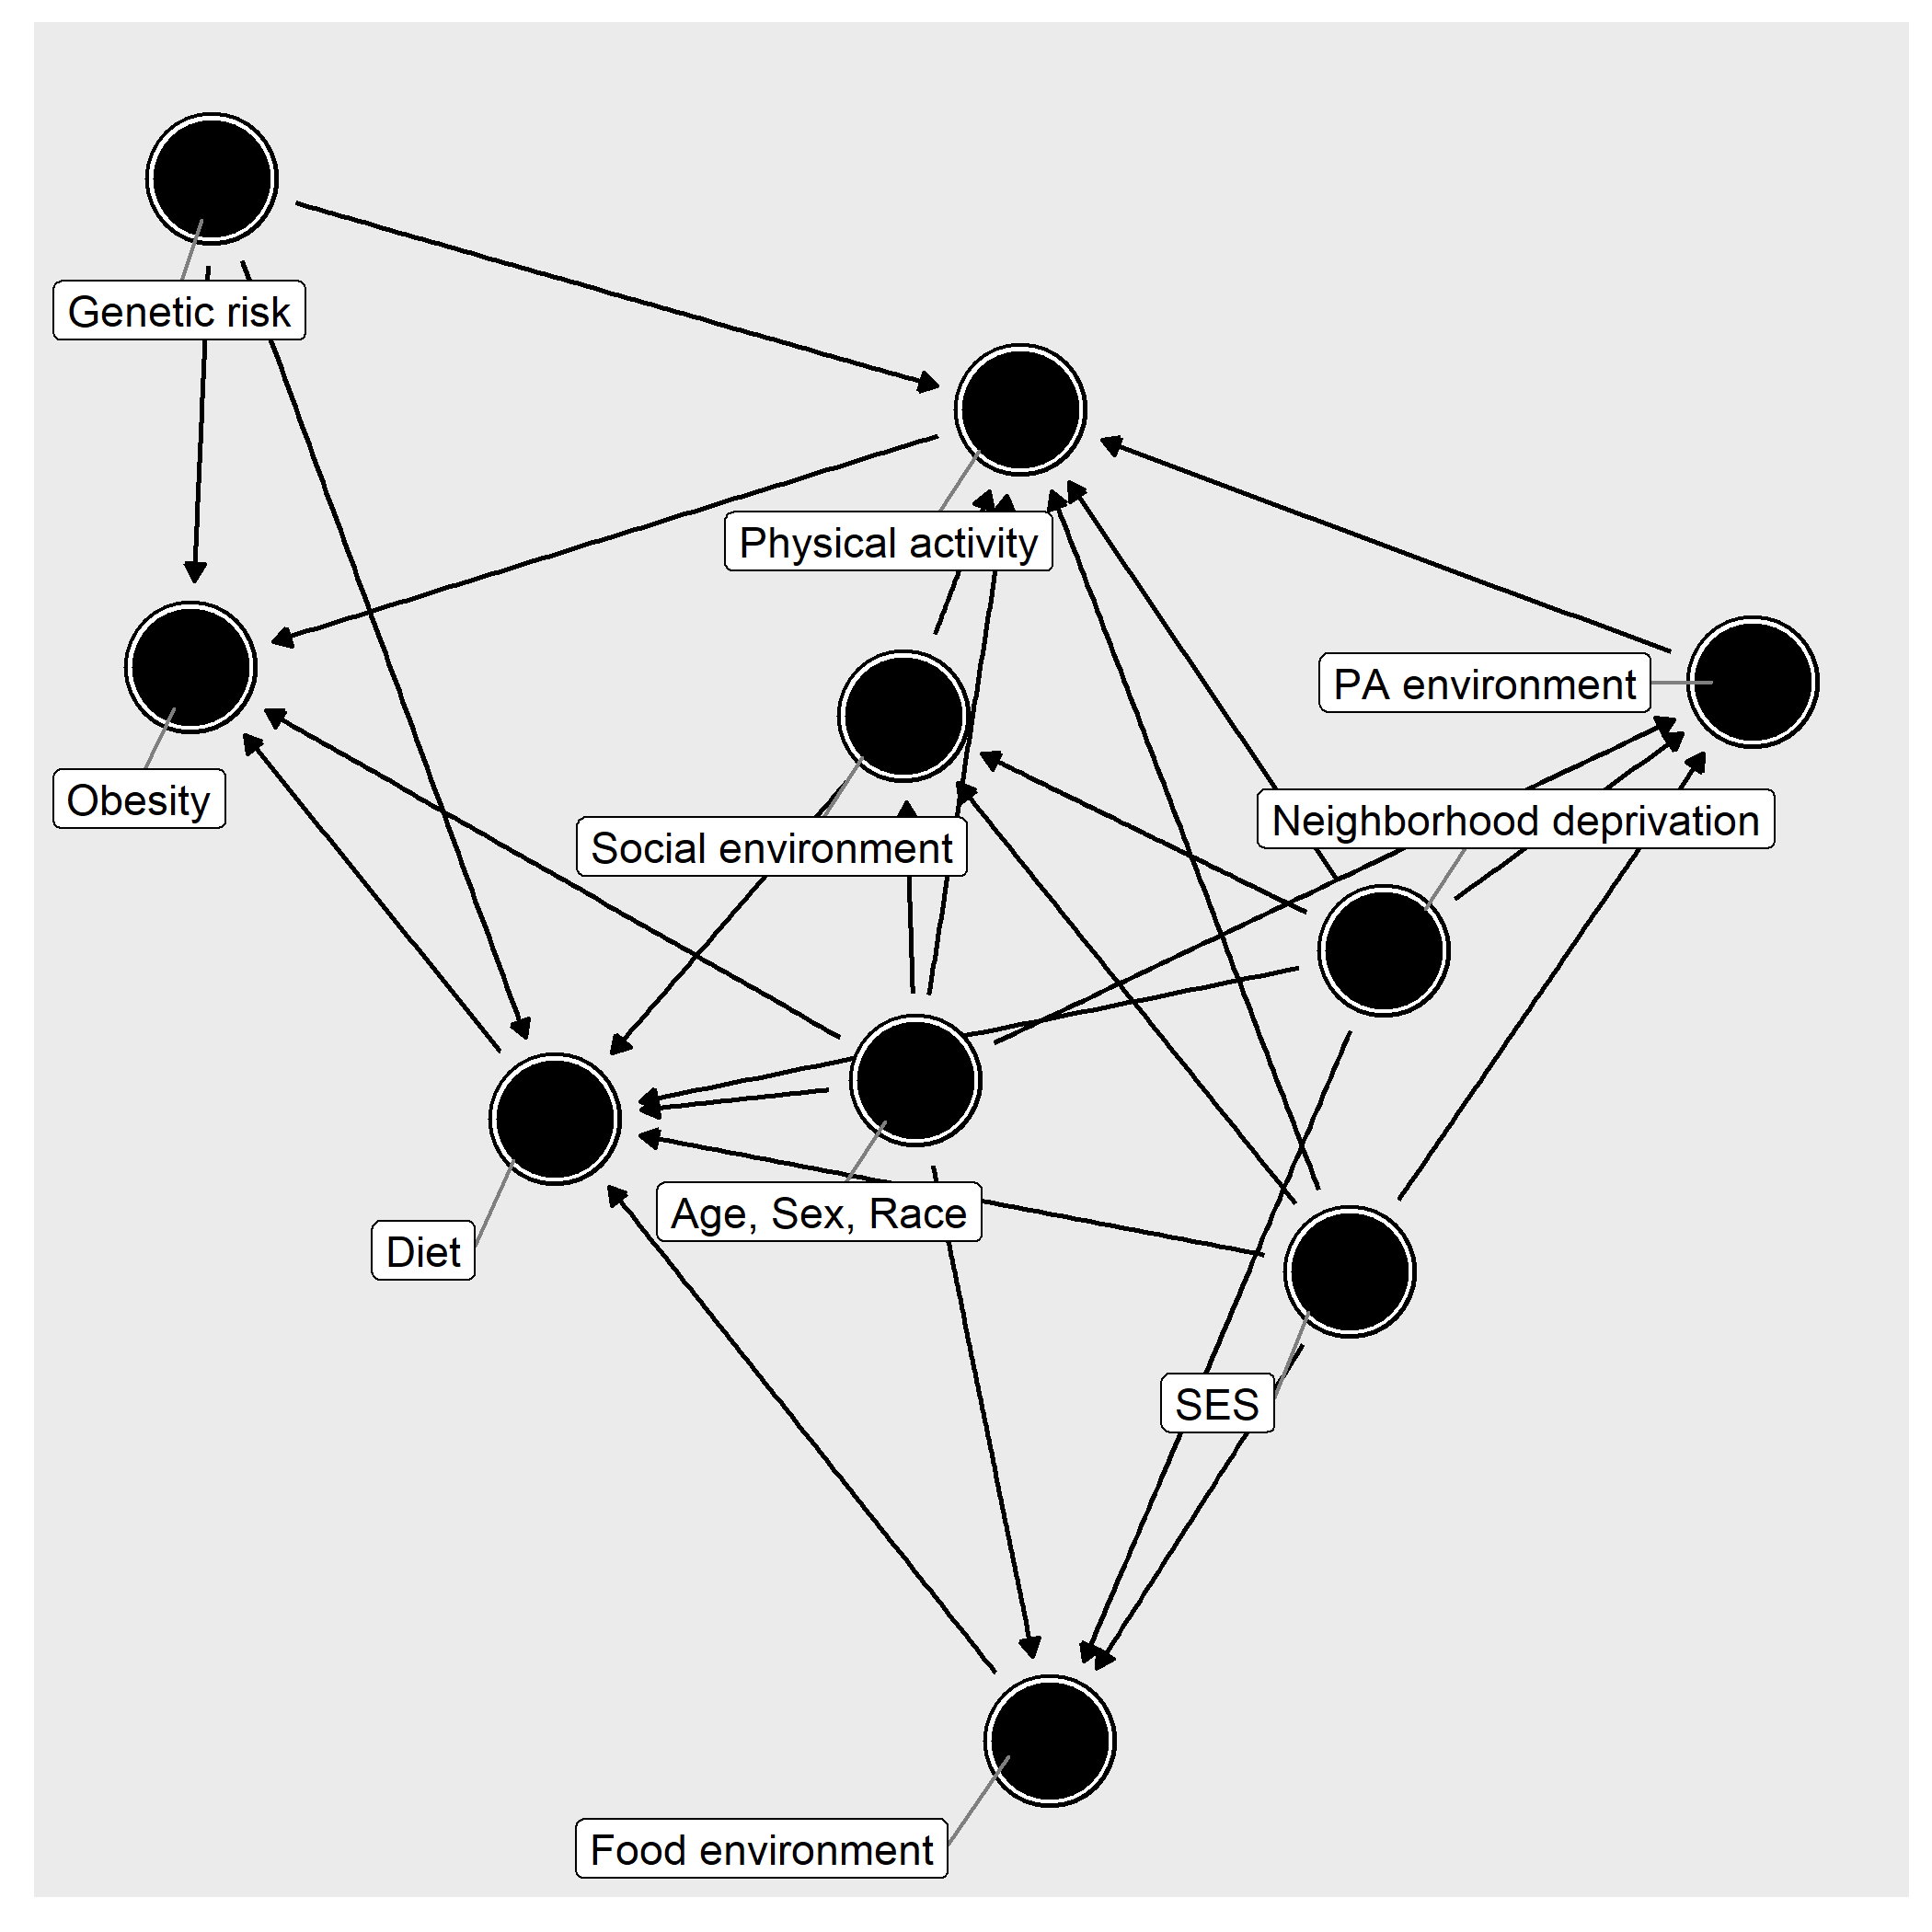
\includegraphics[width=\linewidth]{graph/dag1.png}
\caption{Directed acyclic graph for neighbrhood envrionments and obesity}
\label{fig:dag}
\end{figure}



\newpage

\section{Litterature review}
\subsection{Physical environments}
\paragraph{}
Originally, physical environments have been identified as one of the important determinants on human behaviors based on ecological and socio-ecological model which had evlolved in the late 1900s \cite{mcleroy1988ecological,sallis1998environmental}. Ecological model specifies levels of influence on behavior, from individual, institutional, community, enviornmental, and policy factors \cite{mcleroy1988ecological}. Although there were growing recognitions for the potential effect of environment and policy interventions in the population level, few interventons have been applied to the control of chronic diseases as of late 1900s \cite{schmid1995policy}. It is often challenging to implement environment and policy level interventions as it requires substential investiments and collaborations in various sectors (e.g.health, transportation,and urban planning).

Numerous efforts have been made to put it foward by Sallis et al. specific to physical activity to stimulate more research in this field in order to accumulate sufficient evidences for enviornment and policy changes \cite{sallis1998environmental}. 
\paragraph{}
Since early 2000s, neighborhood research have been accelerated, especially because technologies made it possible to objectively assess physical environment, i.e. geographic information system (GIS). GIS, which used to be utilized in the field of geographics and urban planning to evaluate geography and structure of cities by numerical data, had been incorporated into health field  \cite{frank2005linking}. Collaboration with urban planning and health fields put emphasis on the need of creating "walkable" neighborhoods by focussing on human-made built environments, which had been already recognized for safety perspective, such as Smart Growth America \cite{smartgrowth}.
In several places in the US, environmental interventions to promote healthy behavior had been implemented, such as building public transit or securing walking and cycling infrastructures \cite{brown2015transit,macdonald2010effect}. Although the effects of these interventions have been examined by study design of natural experiments, there are no robust evidences on whether it is effective for reducing the risk of obesity in the population level \cite{tseng2018effectiveness}. Lack of evidences for the association between physical environment and obesity remains as a barrier for implementing enviornmental interventions. 

\subsection{Social capital}
\paragraph{}
Social capital has been defined "features of a social organization, such as trusts, norms, and networks that facilitated cooperation for mutual benefits" \cite{krouwel1995making}. Originally, social capital has been recoginzed as an important determinant for government performance as well as crime prevention and safety \cite{sampson1989community}.It has been found to be an determinant for population health later by Kawachi et al., whose study first identified the association between social capital level and mortality \cite{kawachi1997social}. Since these first studies on social capital, it has been distinguished into "contexual" and "compositional" effects. Compositional effect refers to individual level effect such as having contacts with friends, relatives and family members, or belonging to social groups. Contexial effect refers to group/area level effect such as mutual trusts, supports, and norms within communities. These measures are usually collected via survey or constructed as a proxy by using census data. An important thing to consider is the size of area when measuring social capital. Size of the area could be from minimum of individual to neighborhood, city, state, and countries. When measuring contextual effect of social capital, neighborhood is known to be optimal area size because more rapid diffusion of information occurs within smaller areas compared to larger areas. By integrating these concept and methodology of measuring social capital, a number of research examined the association between social capital and obesity. Carrillo-Alvarez et al. conducted systematic review, and concluded that an association between neighborhood social captial and obesity exits \cite{carrillo2019neighbourhood}. 


\section{Aims and Significance}
\paragraph{Aim 1}
Examining the casual relationship between physical environment and obesity would reinforce the evidence that emphasize the needs of environmental and policy interventions. 

\paragraph{Aim 2}
Examining the effect of physical environment and social environment could infer efficient and cost-effective approach to reduce the risk of obesity.


\newpage

\section{Methods}
\subsection{Aim 1: longitudinal changes of neighborhood physical envionment and obesity}
  \begin{description}
    \item[Study sample] Nationwide sample of men and women from a national Swedish resarch database.
    \item[Analysis] Temporal neighborhood walkability index and proximity to fast food outlets calculated by GIS would be used as primary exposure for obesity. Each exposure would be examined by separete models to predict the effect of each exposure on obesity (Figure 2). For obesity outcome, both continuous BMI and meaningful cutoff point by BMI (e.g. overweight: >= 25, obesity: >= 30) would be used. Potenitial confounding variables such as age, gender, race, income, education, neighborhood deprivation would be controlled (Table 1).  
\begin{figure}[h!]
  \centering
  \begin{subfigure}[b]{0.4\linewidth}
    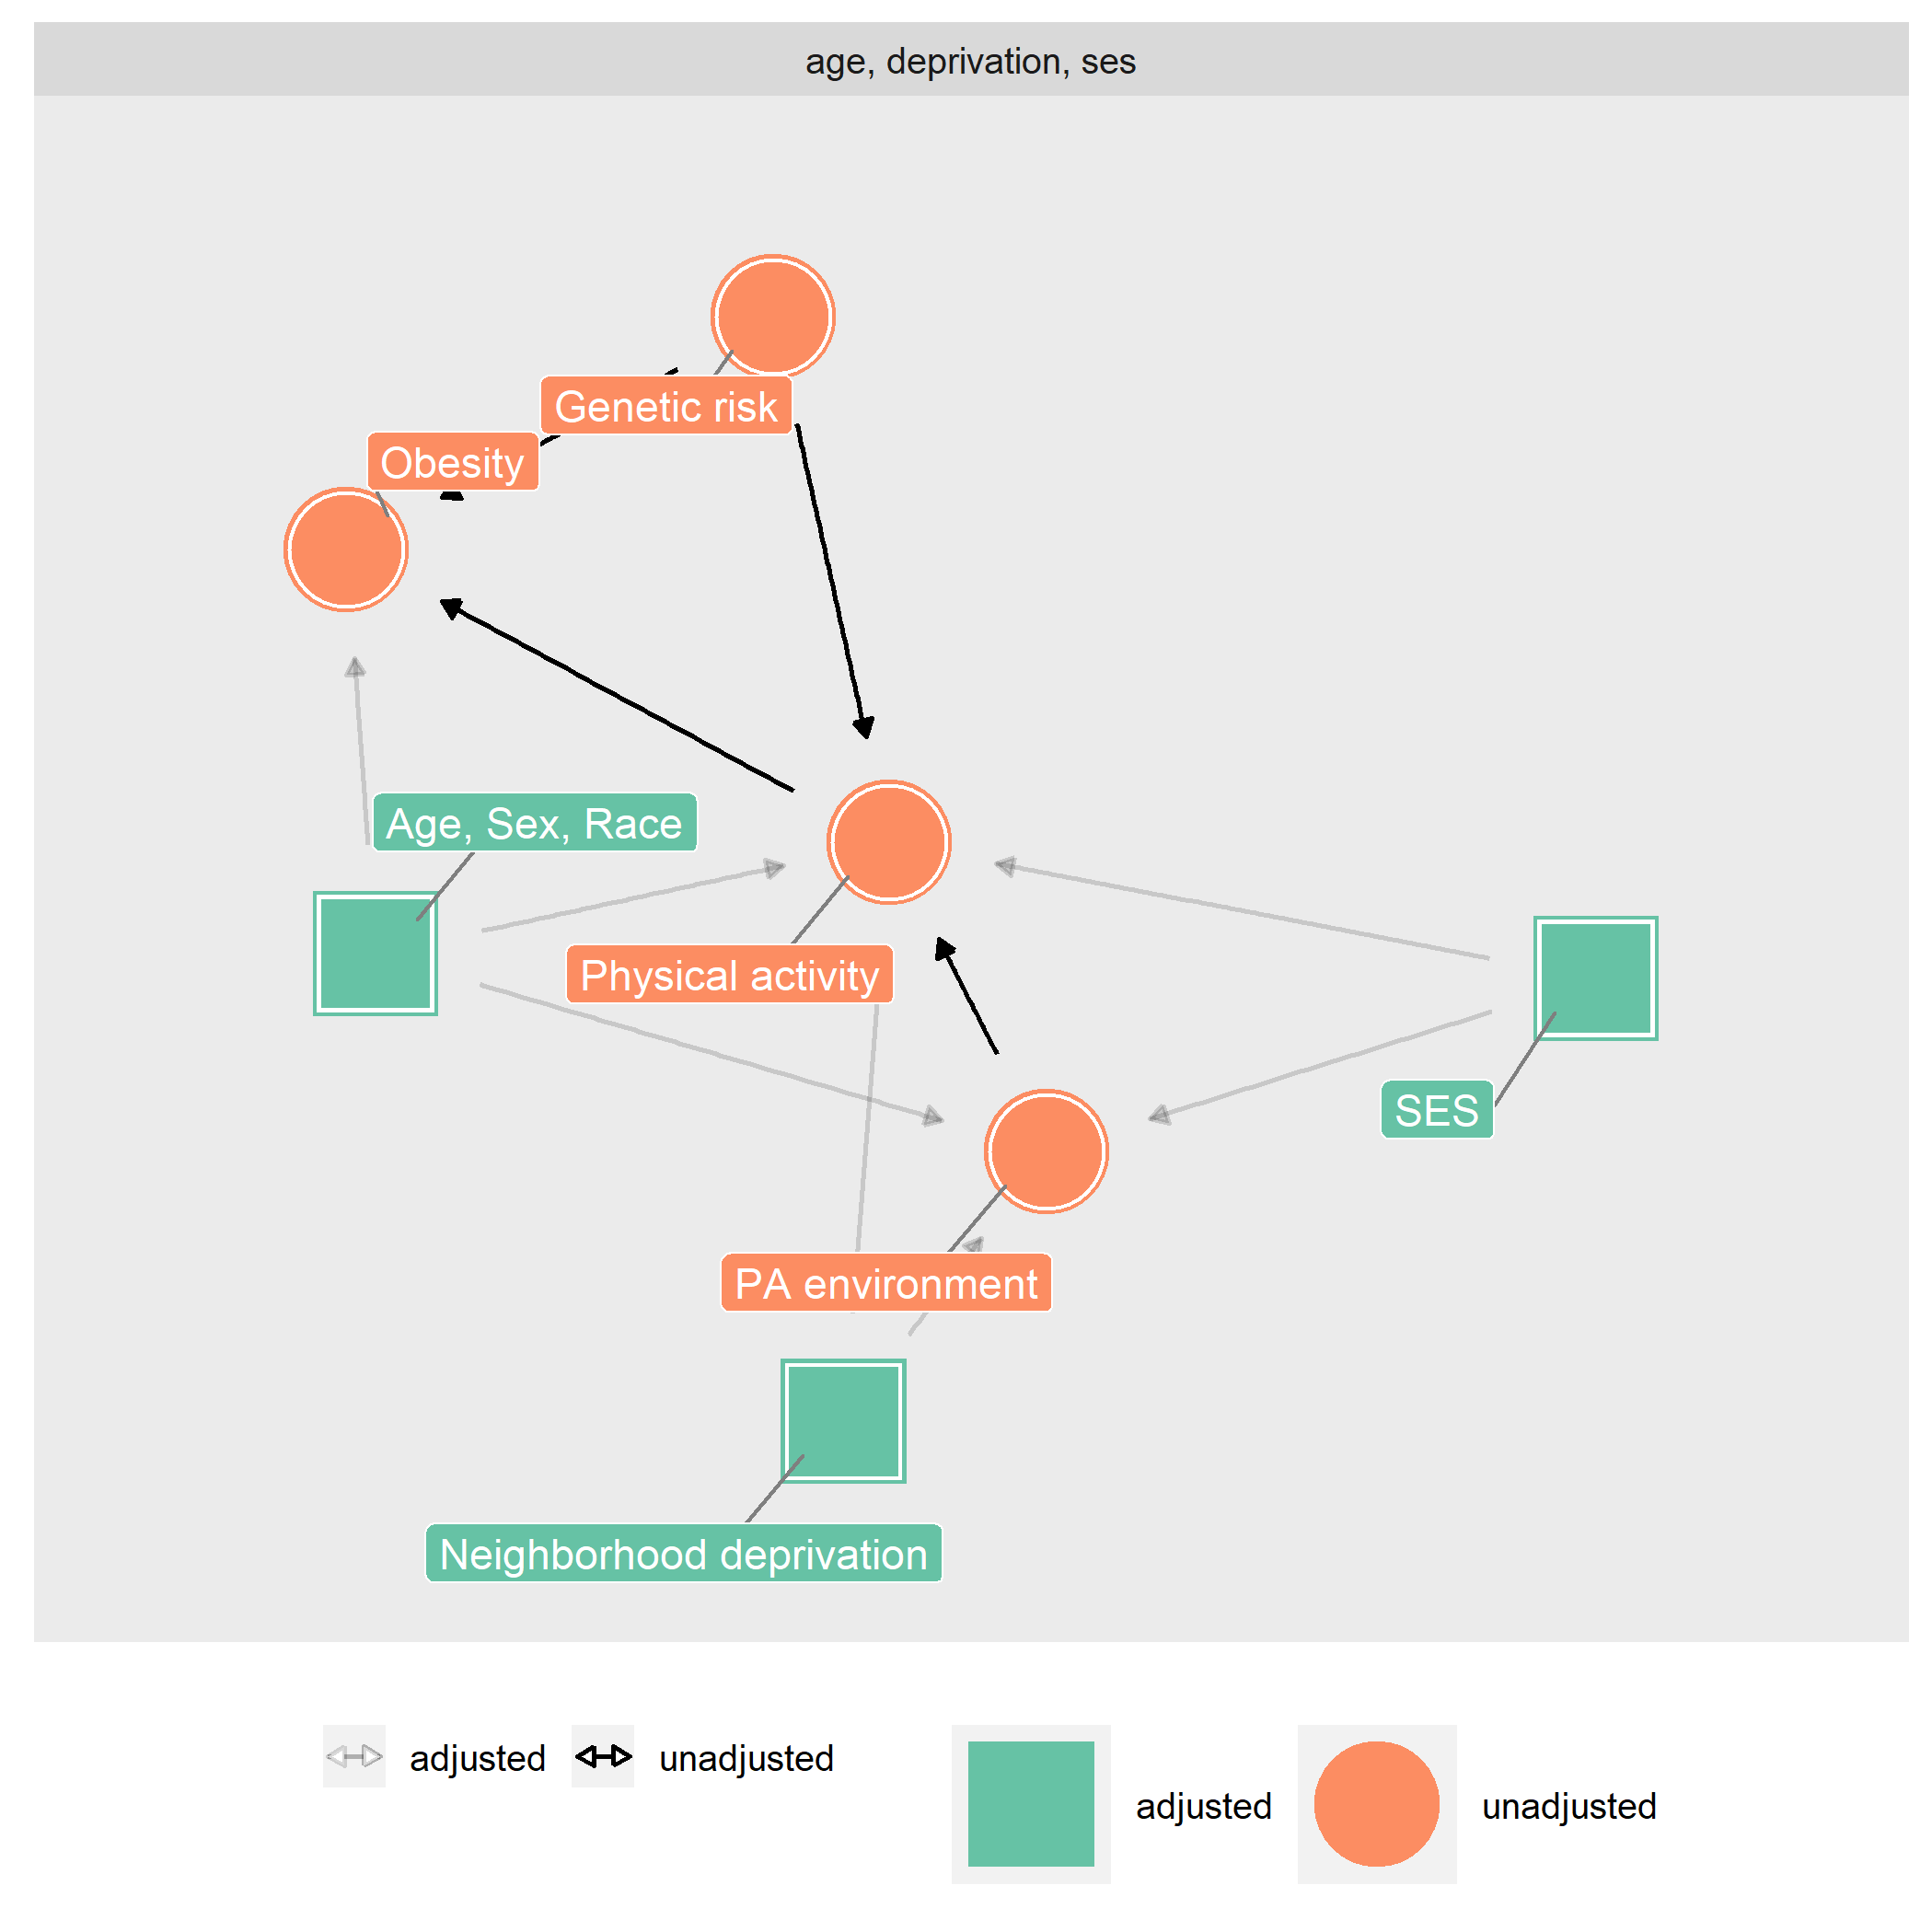
\includegraphics[width=\linewidth]{graph/dag2.png}
    \caption{PA enviornment and obesity.}
  \end{subfigure}
  \begin{subfigure}[b]{0.4\linewidth}
    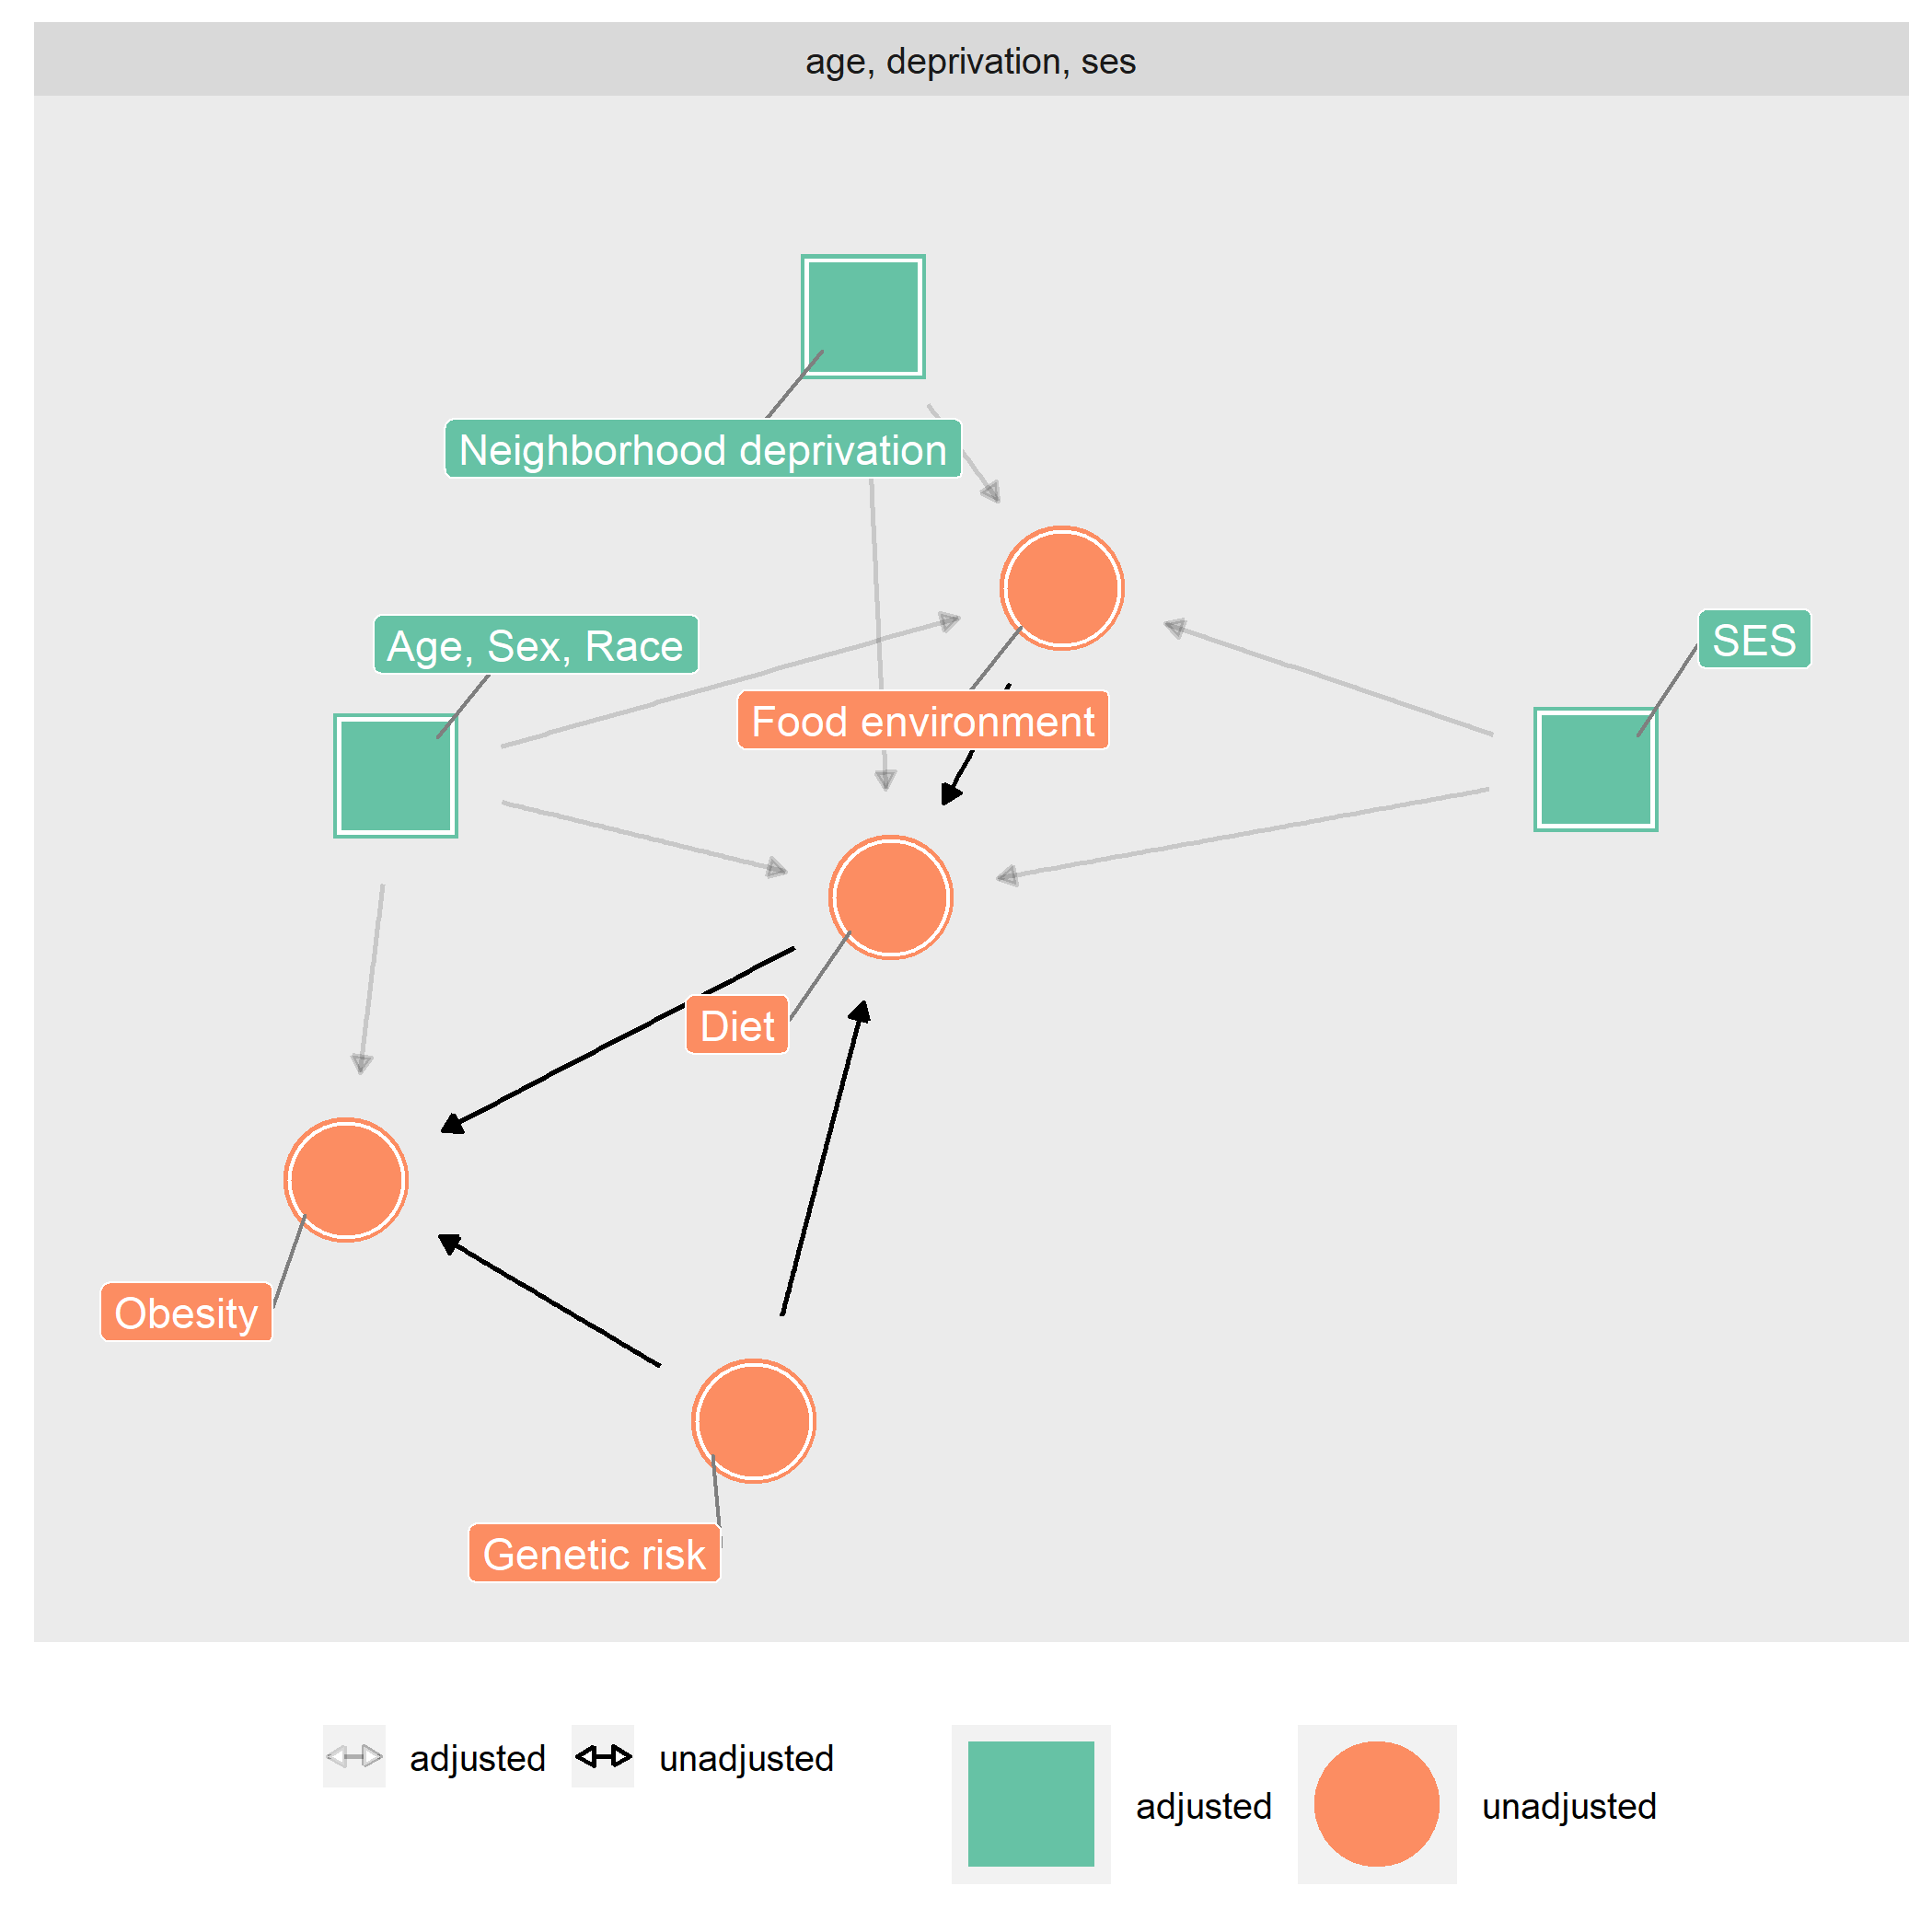
\includegraphics[width=\linewidth]{graph/dag3.png}
    \caption{Food environment and obesity.}
  \end{subfigure}
  \caption{DAG for physical activity and food environment}
  \label{fig:flight}
\end{figure}      

\newpage
	    \begin{table}[h!]
		    \caption{Description of variables to be analyzed}
		    \label{table:aim1}
		      \centering
		      \begin{tabular}{ c l p{5cm} }
			    \hline
			    Type & Name & Description\\
			    \hline \hline
			    Outcome & BMI & Body mass index calculated by objectively measured height and weight.\\
			            & Obesity & Incidence of overweight and obesity defined by BMI cutoff (e.g. >=30).\\
			    Exposure & Food environment & Proximity to fastfood outlets.\\
			             & Physical activity environment & Walkability index which consists of z-score of residential dnsity, land use mix, and street connectivity \cite{sundquist2011neighborhood}.\\
			             
			    Covariates & Basic characteristics & Age, gender, and race. \\
			               & Socio-economic status & Education, and income.\\
				            & Neighborhood deprivation & Neighborhood deprivation index measured by poverty level \cite{kawakami2011differences}.\\
          \hline
			    \end{tabular}
			  \end{table}




\subsection{Aim 2: interaction effect of physial environment and social environment on obesity}
  \begin{description}
    \item[Study sample] Nationwide sample of men and women from a national Swedish resarch database.
    \item[Analysis] Using neighborhood proportion of voting as a proxy for social capital \cite{sundquist2014neighborhood, sundquist2014linking}, examine its effect on adults' obesity and its interaction with physical environment.  
  \end{description}

\newpage

\printbibliography
\end{document}
